%!TEX root = New.tex
\section{Evaluation}
\label{sec:eval}



In this section, we describe our experimental evaluation of \auspice\ on PlanetLab as well as through  trace-driven simulations based on realistic workloads. %We begin with a description of the datasets used to generate workloads.
Our evaluation has three main goals. 
First, is to quantify the performance gap between optimal service placement and heuristic service placement strategies in \auspice.
Second, is to evaluate performance of service placement  schemes in a scenario with high update rates, e.g. a name service for a near future Internet consisting of highly mobile users. 
Third, is to answer whether service placement decisions considering
the geo-distribution of users requests improves performance over
schemes that are agnostic to geo-distribution of users, e.g. \codons. 

%\subsection{Evaluation goals}
%We present an evaluation of the service placement algorithms implemented in \auspice\ on the service workload datasets in Section \ref{sec:datasets}.


\subsection{Replica placement schemes comparison}

In this section, we compare the locality-aware replica placement scheme implemented in \auspice\ against alternate replica placement schemes. In line with our goal of designing a name resolution service for mobile devices in the Internet, we focus on scenarios where a high fraction of name records belong to mobile devices, with each device updating its network address at high frequency. We conduct experiments with the \auspice\ system comparing replica placement schemes on PlanetLab. For larger scale experiments infeasible on PlanetLab, we present results from a simulator that implements the same replica placement schemes.

\subsubsection{Schemes compared}

\textbf{\locaware} refers to the locality-aware replica placement scheme implemented in \auspice. 

\textbf{\uniform} selects the number of replicas using the same heuristic as \locaware\ (Section \ref{sec:heuristic}). The replica locations are chosen randomly instead of being chosen based on geo-locality of the requests.

\textbf{\staticthree} is our baseline scheme. \staticthree\ creates three active replicas for a name at the same locations as the three primary replicas.

\textbf{\codons} is an  alternative DNS architecture implemented on top of Pastry DHT. \codons\ replicates a name record based on its popularity ranking, with more popular name records replicated at greater number of  locations.  The location of replicas is decided by consistent hashing.
Our \codons\ implementation retains these features.
However, we do not implement multi-hop DHT routing used in \codons.
Each request is directly sent to the replica  that would have received this request if Pastry DHT routing were followed.
We achieve this behavior by copying the Pastry routing table of every node at all other nodes and simulating multi-hop routing locally.
Therefore, our latency numbers are a conservative estimate of the latency in \codons. 

\textbf{\replicateall} replicates all name records at all locations.

\textbf{\opt} decides replica locations using the optimization formulation in Section \ref{sec:design}. \opt\ serves as a benchmark for comparison and is implemented only in the simulator. At Internet scale, \opt\ is impractical because of the challenges in solving the optimization problem for billions of name records. 



\subsubsection{Workload}

Our workload consists of a sequence of requests  of name records by clients and updates to name records by the clients that own name records. We distinguish among name records that correspond to today's DNS name records,  called \emph{regular names}, and name records for mobile devices, called  \emph{mobile names}. 

Our workload for regular names are generated based on traffic statistics for websites reported in Alexa Web Information Service \cite{alexa} (AWIS) datasets. AWIS datasets report the relative popularity of each website and the geo-distribution of websites popularity at city-level granularity. 
Across different experiments, we generate a workload based on top-1K, top-10K, and top-100K most popular websites in this dataset. 
The number of updates to name records of a regular names are less than 1\% of the number of queries in the workload. This choice is consistent with the slow rate of change to name records in DNS today.


We generate a synthetic workload for mobile names due to lack of real world datasets. 
The number of mobile names from a country is chosen proportional to its population, an assumption backed by the huge growth in smartphones worldwide. 
We expect the requests for  records of mobile name to show high geographic locality.
The network address updates of mobile devices will be generated by the device itself,  whose mobility is going to be confined to a small geographic region in most cases.
Similarly, a small set of clients will query for a single mobile name, e.g., a user's friends contacting the user's mobile device to send messages, or a mail server contacting a mobile phone to send a push email notification. 
The frequency of queries of mobile names will depend on how applications are designed in future. If applications continue to use a "pull" mechanism as they do in today's Internet, queries for mobile names are likely to be small. However, if most applications switch to a "push" mechanism enabled by \auspice, queries for mobile names will be higher. 
We study the two scenarios by varying the query rates for mobile names in our experiments.


\subsubsection{PlanetLab deployment}


\begin{figure}
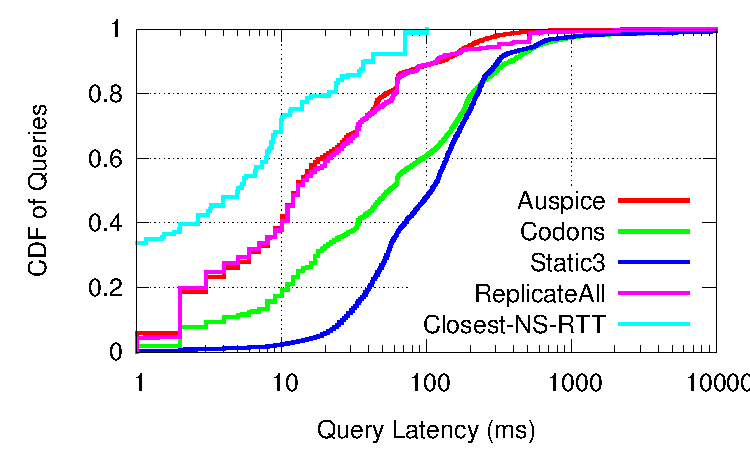
\includegraphics[scale=0.6]{graph/system-exp/cdf-comparison.pdf}
\caption{CDF of latency of all queries.}
\label{fig:querylatencycdf}
\end{figure}

\begin{figure}
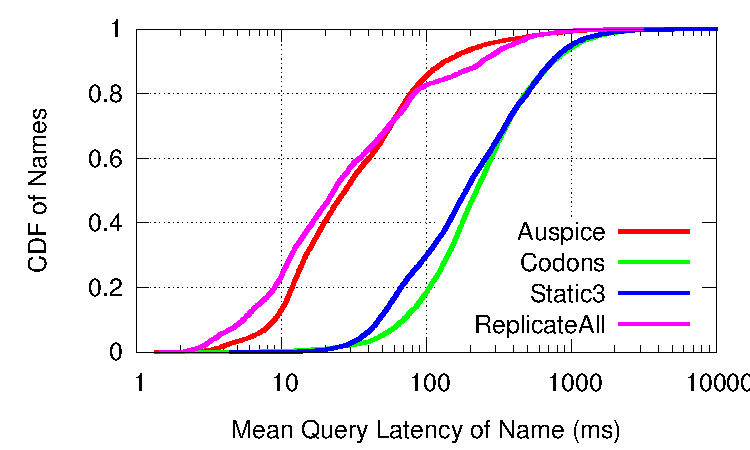
\includegraphics[scale=0.6]{graph/system-exp/cdf-names-mean.pdf}
\caption{CDF of mean latency of queries for all names.}
\label{fig:namesquerymeancdf}
\end{figure}

\begin{figure}
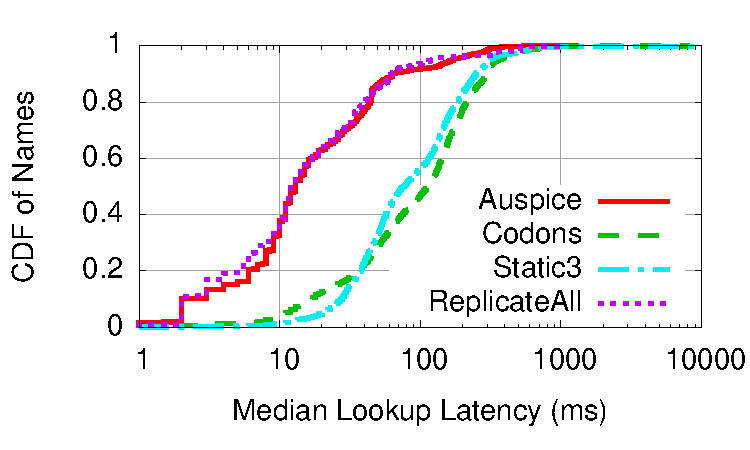
\includegraphics[scale=0.6]{graph/system-exp/cdf-names-median.pdf}
\caption{CDF of median latency of queries for all names.}
\label{fig:namesquerymediancdf}
\end{figure}

%\begin{figure}
%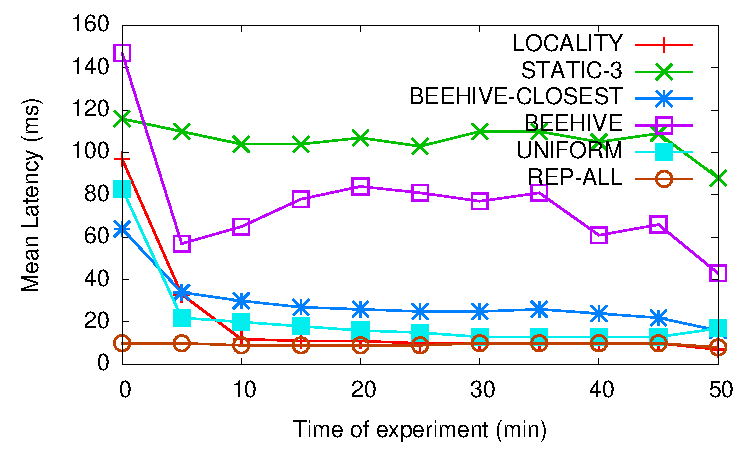
\includegraphics[scale=0.6]{graph/system-exp/timeline-median.pdf}
%\caption{Latency of queries over time. Each point shows the median latency of queries that arrived in the next five minutes.}
%\label{fig:medianlatencytime}
%\end{figure}


Our PlanetLab deployment was done on 160 nodes, 80 nodes running the NameServer module and 80 nodes running the LocalNameServer module. Clients are co-located on the nodes running the LocalNameServer module. If PlanetLab nodes are selected randomly, most nodes chosen are either in North America or in Europe. We use a simple heuristic to select PlanetLab nodes spread across the world.
For each user-group, the geographically closest LocalNameServer location is chosen as its proxy location, e.g., 80 PlanetLab locations  act as a proxy for nearly 15000 cities.  Every LocalNameServer periodically measures the latency to all NameServer locations by running the ping tool. These measurements are used in selecting the closest active replica to send a request.

Our workload consists of requests for 11 K names. Of these, 1 K names are regular names whose requests are generated based on traffic statistics for Top-1K websites in AWIS dataset. Remaining 10 K names are mobile names. The number of queries is 440 K of which 380 K queries are for regular names and 60 K requests are for mobile names; the number of updates  is 420 K, of which only 4 K updates are for regular names and 416 K updates are for mobile names.  The requests in the workload are sent over a duration of 50 minutes. TTLs are set to zero in this experiment. TBD: Why?


Locality-aware replica placement is configured by setting the replication parameter $\alpha$ = 1. This value of $\alpha$ implies that, in this experiment,  a NameServer will receive less than 4 requests / sec  on average (as per Equation 14), which clearly is less than the actual capacity of server. Thus we have made a conservative choice in selecting the replication parameter.  A higher alpha value will create more replicas and will likely lower the query latency. The parameters for \codons\ are set to the same values as described in their paper \cite{codons}.


Figure \ref{fig:querylatencycdf} plots the CDF of latency of queries of every scheme in this experiment. A limitation of Figure \ref{fig:querylatencycdf} is that the distribution is biased towards the more popular names in the workload. We expect a global name service to provide low latencies for all names and not just the most popular names. So, we compare the CDF of mean  latency of queries for each name in the workload in Figure \ref{fig:namesquerymeancdf}. Figure \ref{fig:namesquerymediancdf} compares the CDF of median latencies of queries for each name.  To evaluate the steady-state performance of all schemes, the latency of initial 25\% of queries are not included in these graphs.


% comparison of locality and uniform
Locality-aware placement helps \locaware\ achieve a better performance than \uniform.
The median latency of  \uniform\ is higher than \locaware\ by 40\%, 200\%, and 350\% in Figure \ref{fig:querylatencycdf},  Figure \ref{fig:namesquerymeancdf} and Figure \ref{fig:namesquerymediancdf}  respectively. 
\locaware\ creates the same number of replicas as \uniform, but it creates them close to the pockets of demand resulting in lower query latency. 
The benefit of locality-aware placement is greater for mobile names than for regular names.
Regular names have a high ratio of (read rate) / (write rate), hence both \uniform\ and \locaware\ create a large number of replicas of regular names. 
For this reason, locality-aware placement of replicas provides less benefits to \locaware\ over \uniform\ for queries belonging to regular names, that constitute 86\% of all queries. 
The (read rate) / (write rate) ratio of mobile names is less than 1, hence only one active replica is created for mobile names. The \locaware\ scheme achieves a lower query latency than \uniform\ by placing an active replica in a locality-aware manner. Since 89\% of names are mobile names, this also explains why \locaware\ shows high gains over \uniform\ when CDFs across names are compared.

%We find that the \locaware\ scheme achieves a lower latency than all schemes except the \replicateall\ scheme. 




% comparison of locality and replicate all
The \replicateall\ scheme does achieve a lower latency than \locaware\ but \replicateall\ creates 7.15$\times$ more replicas than \locaware\ or \uniform\ in this experiment. \replicateall\ is not a practical scheme for a global name service because each node must handle all updates. The aggregate update rate of a global name service  will exceed the capacity of a single node which will result in poor performance. To validate this claim, we performed a experiment on a cluster environment with an aggregate update rate of 2750 req/sec in which \replicateall\ scheme resulted in a worse query latency than  \staticthree\ and \locaware.

% poor performance of codons
We find that the \codons\ performs poorly, incurring a higher latency than the baseline \staticthree\ scheme in Figure \ref{fig:namesquerymeancdf} and in Figure \ref{fig:namesquerymediancdf}. 
The higher latecy comes even though \codons\ creates 3.25$\times$ more replicas than \staticthree. 
The number of replicas created is only 14\% less than \uniform.
The poor performance is because DHT routing redirects queries to a randomly chosen active replica instead of the closest active replica of the name, except for names that are replicated at all locations.
\codons\ replicates 3.4\% of most popular names at all locations, and queries for these names achieve low latency; queries for remaining 96.8\% of names result incur high latency.
\codons's strategy achieves good load balancing under heavy load scenario. In a moderate load scenario, load-balancing results in poor latencies.




%(2) Codons scheme performs well for names it replicates every where, for other names in most cases it performance is worse than Static-3 which replicates names. Focus on load balancing results in poor latencies. If we compare latency across names, its performance is the worst.

%(3) The difference between Uniform and Locality shows the value of placing replicas in a locality-aware manner.

%(4) Compare the number of replicas: locality creates less replicas than beehive and  uniform scheme. 

%
%
%Write performance: 
%
%Write latencies are comparable. 




\subsubsection{Simulator}


\subsection{Comparison to DNS \& DNS-Alternatives}


\subsection{Mid-session mobility}


\subsection{}

\subsection{Experimental setup}

\subsubsection{Datasets}
\label{sec:datasets}

{\bf Alexa Web Information Service:}
The Alexa Web Information Service \cite{alexa} (AWIS) provides traffic statistics for websites collected via web crawls and web usage reported by Alexa Toolbar users.
We have collected (after paying a nominal fee) traffic statistics for the top 10000 websites from AWIS. We generate a DNS workload using 
 two statistics from AWIS reports:
(1) PgViewPct: the fraction of page views for each website of all the page views in the Internet.
(2) CityPgViewPct: the fraction of page views from each city for a website of all the page views of the website.
We  assume that the number of requests for a website's name record is proportional to its page views.
%In our workload, total number of requests of a website's name record  is proportional to its PgViewPct.
In our workload, the number of requests from each city of a website's name record is proportional to the PgViewPct $\times$ CityPgViewPct.
\footnote{CityPgViewPct is unavailable for TBD-TBD\% of page views for different websites.
We normalize the fraction of page views from each city so that the aggregate page view fractions of all cities sums up to one.} 

{\bf Social networking:}

\subsubsection{Workload}

\textbf{Name service:}  Our name service workload consists of a sequence of requests  of name record of websites by users and updates to the name record by the website owner.
Each service is a naming service for a unique domain name, and each user-group consists of all users from the same city.
The relative query rate of each website's name record from each city is obtained from AWIS dataset (refer Section \ref{alexa}).
AWIS does not report the frequency at which name records are updated for each website.
We assume that each name record has a fixed update rate equal to a random value in the range of 0.1$\times$ to 10$\times$ the average query rate for a name. 
In our experiments, we analyze the effect of a large or a smaller update rate of name records.
TBD: mobile names
%
%Our name service workload considers each name as a separate service. 
%
%S: For name service workload, each website's name record is a separate service.
%
%$R_{us}$: query rate at user-group u.
%
%$W_s$: Defined in terms of average query rate of a service. Default : 0.1x - 10x of average read rate for a name. 
%

\textbf{Social networking service:} 

%\subsection{Experiment procedure}

\subsubsection{Testbed configuration}

\textbf{Planetlab:} We deploy and evaluate \auspice\ on the PlanetLab testbed. Planetlab nodes are located across six continents which ensures geographic diversity of service replica locations. 
We select 50 Planetlab nodes that act as service deployment locations and 100 Planetlab nodes that act as proxy locations for user groups.
For each user-group, the geographically closest Planetlab location is chosen as its proxy location, e.g., for the name service workload 100 Planetlab locations  act as a proxy for nearly 15000 cities.
Each Planetlab node acting as a proxy location for user-groups measures the latency to all server locations by running the ping tool and vice-versa. \auspice\ decides service replica placements based on these latency measurements. 

%These measurements  input to the service placement algorithms in \auspice.
%
%\auspice\ decides service replica placements based on user to server latency values for all websites. 
%
%These measurements serve as user to server latency 
%
%\auspice\ decides service replica placements based 
%
%These measurements  input to the service placement algorithms in \auspice.

%U: Select 100 local name servers while selecting a minimum 10 from each continent.  Map each user to the PL node that is closest. Each PL node serves as a proxy location for all users mapped to this node.
%
%D: Select 50 = name servers while selecting a minimum 5 from each continent. Set of geo-distributed service deployments.
%
%$L_{ud}$: Ping latency between PlanetLab node and Local name server node. 
%
%$C_d$: equal capacity at all name servers. Capacity of a name server = M * (total read rate of all names + K * total write rate of all names) / (number of name servers).



\textbf{Simulator:} In our experiments with the simulator, we deploy servers at the same locations as the PlanetLab, which ensures similar geo-diversity of service replicas. 
The latency between servers and a user-group is calculated based on the geographic distance between the server location and a representative location for that user-group.
For our name service workload, we obtain representative location's coordinates for each user-group  by geocoding the corresponding city using Google's geocoding service.  
TBD. What about Twitter workload?



%U: Set of cities in the Alexa trace as well as the Twitter trace. Map each user to the PL node that it is closest to. Each PL node serves as a proxy location for all users mapped to this node.
%
%D:  Set of geo-distributed service deployments.
%
%$L_{ud}$: Latency proportional to geo-distance between user's location and each  server
%Ping latency between PlanetLab node and Local name server node. 


%\subsubsection{\auspice\ configuration}
\subsubsection{Compared placement algorithms}

\auspice\ runs three replicas of every service to ensure fault tolerance. 
The location of service replicas is updated once every 10 minutes.
Our evaluation scenarios do not consider time varying workloads but \auspice\  is designed to update service replica placement with as workloads change over time.

All algorithms in \auspice\ provide a trade-off between the user-perceived latency  and the server load by varying a single parameter, 
e.g. increasing the multiplier constant $M$ for \locaware\ creates more service replicas and reduces latency. 
We evaluate every scheme  for a wide range of parameter values and record the mean latency and the mean server load in each case.
We aggregate results for all parameter values on a single chart that plots the average server against average server latency.
This draws out the tradeoff between latency and server load for every scheme and is used to  compare different schemes.
We vary the multiplier constant $M$ for \locaware, \kmedoids, and \uniform\ schemes.
For \opt, we vary the server capacity $C_d$   at each server. 
And we vary the parameter C in  \codons\ that determines the average number of hops each request traverses in an overlay routing.

\subsection{Lookup performance}

Figure 1: (a) latency CDF across regular names
(b) latency CDF across mobile names
(c) latency CDF across 1 regular names and 10 mobile names

Figure 2: mean/median latency as  a function of \% mobile names

Figure 3: (a) latency VS read load (both regular and mobile)
(b) latency VS write load (both regular and mobile)

Figure 4: update cost vs  read/write load (number of replicas $\times$ update rate)

Figure 5: (a) load balance as a function of read load
(b) load balance as a function of write load

1(a)(b)(c) 10000regular names, number of requests: 10,000,000
read rate: regular names: 1/TTL
mobile names: 1-10 req/day
write rate: regular names: 0.1 - 1 of read rate
mobile names: 10-100 req/day

number of LNS 100, number of NS: 100
locality of mobile names: each mobile name is read randomly from 5 closest LNSs
 
First graph: Latency CDF across all names (e.g. Figure \ref{fig:lookup1})

\begin{center}
\line(1,0){240}
\end{center}

{\bf Default setup for the first graph:}

(1) {\bf Number of names:} 
100K regular names, 1M mobile names

(2) {\bf Number of requests:} 
90\% of total requests are for regular names, and 10\% are for mobile names.

(3) {\bf Read rate:}  

Regular names are generated according to Alexa popularity, total number of regular requests and experiment duration, not TTL.

Mobile names are generated uniformly between 1 and 10 requests per day

(4) {\bf Locality:} 

Regular names are generated according to Alexa data.

Each mobile name is generated randomly from between 1 and 5 local name servers that are within the same country.

(5) {\bf Update rate:}

Regular names: 0.01 and 0.1 of mobile name writerate

Mobile names are updated uniformly between 10 and 100 requests per day

(6) {\bf Number of replicas:}

UNIFORM and LOCALITY: TBD\_parameter $\times$ readrate/writerate

BEEHIVE: tune its averagehopcount parameter so that the average number of replicas across all names is the same as that of UNIFORM and LOCALITY

\begin{center}
\line(1,0){240}
\end{center}

Second graph: latency as read load increases (e.g., \ref{fig:lookup2})

Third graph: latency as write load increases: similar to \ref{fig:lookup2}


\begin{figure}[t]
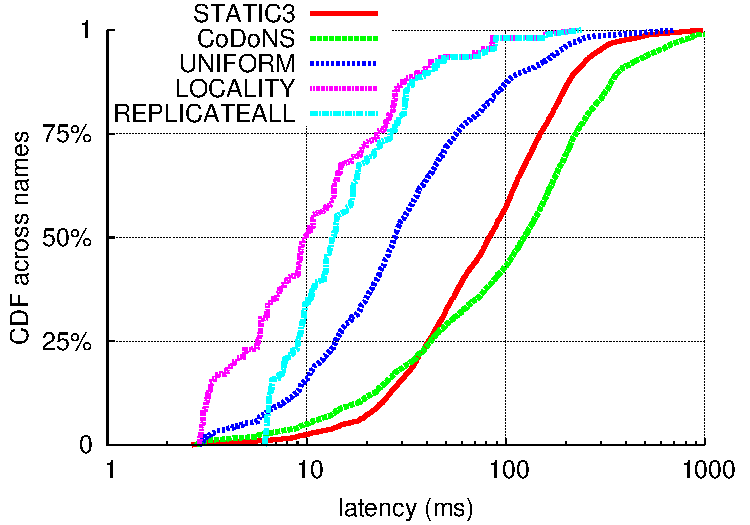
\includegraphics[scale=0.6]{graph/latencycdf.pdf}
\caption{Latency CDF for 10000 regularnames}
\label{fig:lookup4}
\end{figure}

\begin{figure}[t]
\includegraphics[scale=0.6]{graph/meanlatencyVSload5.pdf}
\caption{Mean latency vs load for 10000 regular names}
\label{fig:lookup1}
\end{figure}

\begin{figure}[t]
\includegraphics[scale=0.6]{graph/medianlatencyVSload5.pdf}
\caption{Median latency vs load for 10000 regular names}
\label{fig:lookup2}
\end{figure}

\begin{figure}[t]
\centering
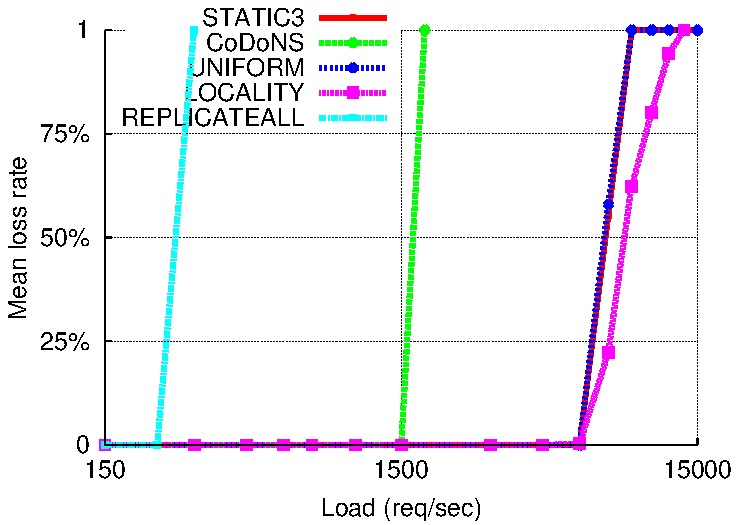
\includegraphics[scale=0.6]{graph/lossrate.pdf}
\caption{Lossrate vs load for 10000 regular names}
\label{fig:lookup3}
\end{figure}

\subsection{Update cost}

Figure \ref{fig:lookup3} by varying the number of replica parameters to get different number of replicas


\subsection{Load balance}

Plot fairness and latency

\subsection{Others}

Vary the percentage of requests for regular and mobile names

%\subsection{Social Networking Service}
%\label{sec:twitter}

%Fourth experiment: Similar graphs as Figure \ref{fig:dns1} and Figure \ref{fig:dnsupdate}.


%\subsection{Akamai Edge Computing Workload}
